% The original numerical line and analytic CDF are embedded unchanged.
\begin{tikzpicture}[textbook diagram]
  \node[inner sep=0,anchor=south west] (plot) at (0,0) {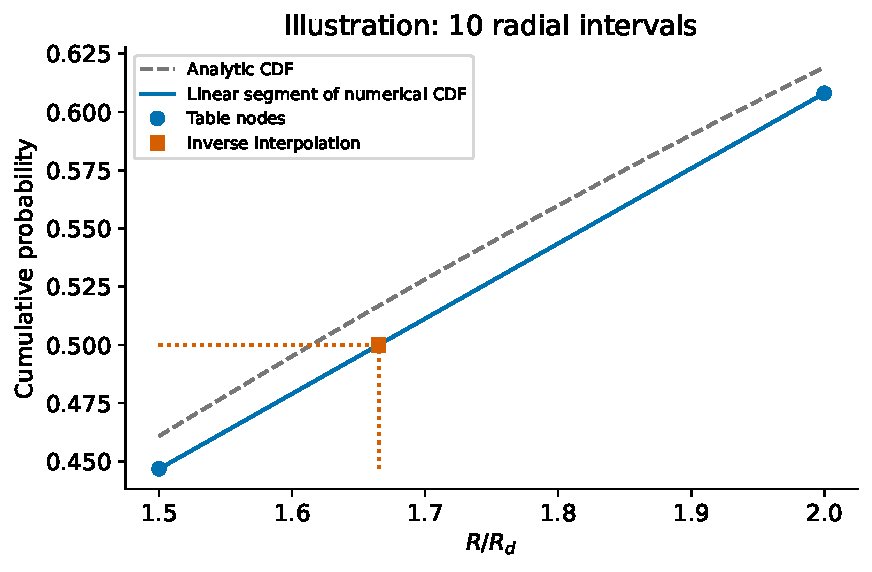
\includegraphics[width=118mm]{figures/ch04_interpolation.pdf}};
  \begin{scope}[x={(plot.south east)},y={(plot.north west)}]
    \draw[vector,figred] (.147,.396700) -- (.422,.396700);
    \draw[vector,figred] (.433970,.380) -- (.433970,.146);
    \node[small label,fill=white,inner sep=1pt,above] at (.245,.402) {$u=0.5$};
    \node[small label,fill=white,inner sep=1pt,anchor=west] at (.453,.196) {$\widehat R(u)/R_d$};
    \node[small label,fill=white,inner sep=1.5pt,anchor=west] (lo) at (.24,.198) {$(R_j,\widehat F_j)$};
    \draw[guide] (lo.west) -- (.182204,.180028);
    \node[small label,fill=white,inner sep=1.5pt,anchor=east] (hi) at (.905,.545) {$(R_{j+1},\widehat F_{j+1})$};
    \draw[guide] (hi.east) -- (.944684,.836223);
  \end{scope}
\end{tikzpicture}
